\documentclass[12pt,a4paper,IEEEtran]{article}
\usepackage[utf8]{inputenc}
\usepackage{array}
\usepackage{amsmath}
\usepackage{amsfonts}
\usepackage{amssymb}
\usepackage{graphicx}
\usepackage{booktabs}
\usepackage{algorithm}
\usepackage{algpseudocode}
\usepackage{subcaption}
\usepackage[english]{babel}
\usepackage[export]{adjustbox}
\usepackage{enumerate}
\usepackage[left=3.5cm,right=2.5cm,top=2.5cm,bottom=2.5cm]{geometry}
\usepackage{lineno}
\usepackage{cite}
\usepackage{acronym}
\renewcommand{\baselinestretch}{1.5}



\begin{document}

	\begin{center}
		\begin{LARGE}			\bf{Topic Name / Title\\}
		\end{LARGE}
		\vspace*{30pt}
		\textbf{Applied Digital Image Processing \\ Fall 2023}
		\vspace{40pt}
		
		\textbf{
			Shayan Shoaib Patel (Student ID: sp07101)\\
			Muhammad Areeb Kazmi (Student ID: mk07202 )\\
            Group 12}\\

		\vspace{30pt}
		
\includegraphics[width=0.3\textwidth]{./logo.png} \\
		\vspace{30pt}
		\textit{Under the kind guidance of}\\
		\textbf{Dr. Muhammad Mobeen Movania}\\
		\textit{\textbf{Assistant Professor, Computer Science}}
		
		
		\vspace{20pt}
		
		
		\textbf{Dhanani School of Science And Engineering\\
			Habib University\\
			October 24, 2023
		}
	\end{center}

\pagenumbering{arabic}

% Every latex document starts with a documentclass declaration like this
% The option dvips allows for graphics, 12pt is the font size, and article
%   is the style

%\usepackage[pdftex]{graphicx}
%\usepackage{url}

% These are additional packages for "pdflatex", graphics, and to include
% hyperlinks inside a document.

\setlength{\oddsidemargin}{0.25in}
\setlength{\textwidth}{6.5in}
\setlength{\topmargin}{0in}
\setlength{\textheight}{8.5in}

% These force using more of the margins that is the default style


% Everything after this becomes content
% Replace the text between curly brackets with your own


% You can leave out "date" and it will be added automatically for today
% You can change the "\today" date to any text you like


% \maketitle

% This command causes the title to be created in the document
\newpage
\section{Abstract}

\section{Introduction}
% this para is good. 
In the context of our present ecological challenges, addressing and raising awareness about global warming stands as a paramount imperative. Given the limitations in resources and the potential reluctance of governing bodies to prioritize this issue adequately, it becomes essential to pioneer a systematic approach for monitoring, reflecting upon, and mitigating these environmental changes. 

% can be used in significance of the research
Our primary objective is to institute a meticulous process for the collection and analysis of satellite imagery. Subsequently, we intend to apply various advanced methodologies and mathematical algorithms to these images. This multifaceted approach serves a dual purpose: it helps in our ability to fairly analyze and document alterations in land topography brought about by climate change upto an approximate degree, while also diminishing our reliance on local authorities and potential vested interests that may obstruct progress in this crucial area.
% significance

By implementing this approach, we aspire to foster greater transparency, accountability, and data-driven decision-making in the quest to combat global warming. Moreover, this initiative carries the potential to engage and enlighten the public about the pressing need for environmental conservation, ultimately leading to a more sustainable and resilient future for our planet as we try to compare and contrast different classical digital image processing techniques with the current state of the art method.
% An article style is separated into sections and subsections with 
%   markup such as this.  Use \section*{Principles} for unnumbered sections.


% \section{Motivation}
% The motivation behind the proposal is to work with a real world problem which is significant to the survival of human species.
% Deforestation is one of the by-products of the climate change that has contributed to the global warming. Keeping the context of
% the course in mind, we aim to use techniques and knowledge acquired in the course to try to improve the process of identifying deforestation and the effects brought
% by the anthropocene. 
% \newline The satellite technology accompanied with the high=resolution imagery can be a game changer in the monitoring and identification of deforestation and urban expansion.
Our project aims to utilize the capabilities and functionalities of classical digital image processing for the purpose mentioned above that can be done using satellite imagery and images from Google Earth.
% Here are some of the key motivations behind the project:
% \subsection[2.1]{Environmental Impact}
Deforestation is a major contributor towards
the global boiling, as environmentalists term it now (instead of global warming). The monitoring system can contribute towards helping the relevant stakeholders to make better informed decisions through sustainable development. \cite{thomas2023global}

% \subsection[2.2]{Utilizing the true essence of Computer Science}
% To our limited understanding, Computer Science has been the field of study that has been involved in solving problems that exist in the world. In fact, vast collaborations with practitioners, theorists, biologists, chemists, and people of other
% professions have led to the innovation of new tools, applications, and opportunities. The same analogy can be directed towards solving a part of the problem of climate change and deforestation. By deploying suitable machine learning algorithms, image classification, and object detection methods, if possible,
% we might be able to experience the very same essence of CS in this course.
% \newline  
% Apart from the technical aspects, the project will also give us the opportunity to pitch ideas to relevant stakeholders, conduct the various phases of the project by managing it on time, and improve our own skillset and knowledge arsenal.
% This project will help us to make a meaningful impact while gaining invaluable experience in the area of applied digital image processing.

\section{Literature Review}
This section entails a review of the previous work done in the scope of detecting deforestation using different types of satellite imagery. Most of the techniques use remote sensing, i.e., making use of the satellite imagery to detect image change and deforestation. While the methods in section 3.1 and 3.2 work on single band images, section 3.3 and onwards work on multi-band images which is the current state of the art procedure. \\
Our project aims to bring classical techniques and compare their results with the more accurate methods to see if the classical methods can be used to have a fair estimate of the deforestation since the acquisition of multi-band satellite imagery and the pre-processing required is cumbersome and cannot raise public awareness.

%Taken from Paper 3

%Taken from Paper 3

\subsection[3.1]{Image Clustering} 
Content Based Image Clustering (CBIR) is a method used to group or classify objects into different classes which have similar properties. These classifying of images help us study different characteristics of 

This classifying of images into groups help assist study different characteristics of the image like better flow, pattern changes and similarity of events or phenomenon. Further clustering of images gives clusters or regions with detailed and concise information and the content of the images which ease the task of asserting this regions of clusters. 
\newpage The Fuzzy C-Means (FCM) clustering method \cite{BEZDEK1984191} is based on minimizing the following objective function:
\begin{equation}
J_m = \sum_{i=1}^{n} \sum_{j=1}^{c} u_{ij}^m \cdot \|\mathbf{x}_i - \mathbf{v}_j\|^2
\end{equation}
\newline Here's a breakdown of the terms:
\begin{itemize}
    \item $J_m$ is the objective function to be minimized.
    \item $n$ is the number of data points.
    \item $c$ is the number of clusters.
    \item $u_{ij}$ is the degree of membership of data point $\mathbf{x}_i$ to cluster $j$.
    \item $m$ is a weighting exponent, usually set to 2 for FCM.
    \item $\mathbf{v}_j$ is the centroid of cluster $j$.
    \item $\|\mathbf{x}_i - \mathbf{v}_j\|^2$ is the Euclidean distance between data point $\mathbf{x}_i$ and the centroid $\mathbf{v}_j$.
\end{itemize}

The objective is to find the membership values \( u_{ij} \) and cluster centroids \( \mathbf{v}_j \) that minimize the objective function. The degree of membership \( u_{ij} \) indicates the fuzzy assignment of data point \( \mathbf{x}_i \) to cluster \( j \), with higher values indicating stronger membership.


FCM (Fuzzy C-mean) is one of the most common form of image clustering and it is the based on the principle of fuzzy classification. In fuzzy C-mean clustering pixels with identical properties will be grouped into to same categories or clusters. [Cite 2 Doc 22]

The input images of the fuzzy C-mean clustering, where Gray scale images and the cluster centers were computed automatically by the function itself. Once the cluster center was found and fixed, the next stage was setting the rules for fuzziification. That is if-then rules are given below assuming that the three cluster values are cluster 1, 2 and 3.
\begin{itemize}
	
	\item If pixel (i,j) is less than Cluster-1, center make it black(0)
		%\centering
	\item If pixel (i,j) is greater than cluster-3 center make it White (1).
		%\centering
	\item Else make pixel (i,j) in between black and white (0.5). 	
	%\end{flushleft}
\end{itemize}

The FCM algorithm continuously upgrades and moves this cluster centers iteratively to the ideal or right position. So by continuous moving of initial cluster centers, it precisely clusters the image into different regions and groups the accuracy of the membership grades of each groups [Cite3 in 23 in Doc]. 


\subsection[3.2]{Otsu Method on color spaces}
Image Segmentation is seperating or dividing of images into different clusters or regions based on common properties and/or differences between other regons properties. One property out of the many could be applied to separating images into regions is pixel intensity. 

The method involves finding an optimal threshold that minimizes the intra-class variace of pixel intensities:
\begin{equation}
	\sigma^2_w(t) = w_1(t) \cdot \sigma_1^2(t) + w_2(t) \cdot \sigma_2^2(t)
\end{equation}
Where: 
\begin{enumerate}
	\item $t$ is the threshold value.
	\item $\sigma^2_w(t)$ is the weighted sum of the variances of the two classes spearated by the threshold
	\item $w_1(t)$ and $w_2(t)$ are the probabilities of the occurences of the two classes separated by the threshold.
	\item $\sigma_1^2(t)$ and $\sigma_2^2(t)$ are the variances of the two classes separated by the threshold.
\end{enumerate}
The goal here, is to find the threshold value $t$ which effectively spearates the image into two classes, that minimizes the intra-class variance and maximizes the inter-class variance. \cite{5254345}

So we normally can segment images into different regions through thresholding or separating the pixel levels into different scales. These different thresholding scales create different regions corresponding to the pixel intensity values. 
\newline A simple example can be thresholding a gray scale image pixels into two regions, by transforming the gray scale image into binary image, which will consist of only two regions, namely either the black or white.

If $G(x,y)$ is a threshold version of $f(x,y)$ at some global threshold $T$,:
\[G(x,y) =
\begin{cases}
1 & \text{if } f(x,y) \geq T\\
0 & \text{ otherwise}
\end{cases}
\]

This method has been used with color spaces like HSV (Hue, Saturation, Intensity), and L*a*b* to identify areas of deforestation that we will further see in the methodology section.


% paper 2 used

% \subsection[3.3]{Image ratioing}
% Ratioing is considered to be relatively rapid means of identifying areas of change. In ratioing two registered images from different dates with one or more bands in an image are ratioed, band by band. The data are compared on a pixel or pixel basis. 

% \begin{equation}
% R(x) = \frac{I_{1}(x)}{I_{2}(x)}
% \end{equation}

% If the intensity of reflected energy is nearly the same in each image of R(x)=1, this indicates no change. In areas of change, the ratio value would be significantly greater than one or less than one, depending upon the nature of the change between the two dates. 

% Paper 2 used

\subsection[3.3]{Change Vector Analysis}
The change vector analysis \cite{MINU20151366} involves two variables, the magnitude of variation and the angle of the change vector.
The change vector is obtained by subtracting the images represented in vector form.
The first step of the CVA method is to find (Normalized Difference Vegetation Index) NDVI and (Bare Soil Index) BI values of both the images.

\begin{equation} NDVI = (NIR - RED) / (NIR + RED) \end{equation}
\begin{equation}
	BI = ((SWIR + RED) - (NIR + BLUE)) / ((SWIR + RED) + (NIR + BLUE))
\end{equation} 
where $NIR$, $RED$, $SWIR$ and $BLUE$ are the spectral reflectance measurements acquired in the near-infrared, red, short wave infrared and blue regions.
Change vector of each pixel includes two components NDVI and BI, which are the 2 axes in Cartesian coordinate system. The start point and finish point of the change vector are the locations of pixel in NDVI-BI space. The magnitude of vector represents the change intensity and the direction of vector represents the change dimension 
Further calculations not only allow us to furhter divide the values into two different groups which do not only allow to see the land and forestation/plantation affected.

% \subsubsection[3.4.1]{Tasseled Cap Transformation Method}
% The tasseled cap transformation parameters of ETM+ imagery were used to calculate the Brightness, Greenness 
% and Wetness components of each image. The Tasseled cap transformation coefficients derived for Landsat 7 ETM+ 
% data by the EROS Data Center (Huang et al. 2002) are given in Table 2. Brightness is a weighted sum of all bands, 
% defined in the direction of the principal variation in soil reflectance. Greenness is a contrast between the near infrared and visible bands. It is strongly related to the amount of green vegetation in the scene. Wetness relates to 
% canopy and soil moisture. The brightness, greenness and wetness indexes are obtained for both the images.

% \begin{figure}[h]
% 	\centering
% 	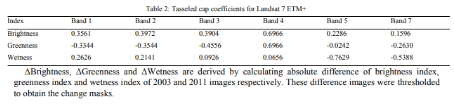
\includegraphics[width=0.7\linewidth]{./tasseledcap}
% 	% \caption{Tasseled Cap Transformation}
% 	\label{fig:tasseledcap}
% \end{figure}

% \subsubsection[3.4.2]{Principal Component Analysis Method}
% The principal components transformation is a linear transformation which defines a new, orthogonal co-ordinate 
% system such that the data can be represented without correlation. A bi-temporal feature space is constructed by 
% placing the two image vectors in the same space. The transformation is found from the eigen vectors of the 
% covariance matrix of the original data. Each individual pixel is transformed by vector multiplication of its original 
% vector and the eigen vectors, resulting in coordinates in the new space. The transformed data is re-arranged back into
% wo images corresponding to the first and second principal components. The first component images contain no change pixels whereas the second component images contain change information between the different dates.

% Therefore, using the Brightness, Greenness and Wetness components of each image, the change vector analysis was performed. 

%Paper 9 used here

\subsection[3.4]{NDVI Method}
This method entails the use of multi-band satellite imagery to detect and produce results for areas of vegetation \cite{isprs-annals-IV-4-W4-379-2017} where the Landsat 8 has eight bands: blue, green, red, near-infrared 1, 
near-infrared 2, thermal, mid-infrared, panchromatic. All of the 
bands have 30 meters resolution, except thermal with 60 and 
panchromatic with 15 meters of resolution (GIS Geography, 
2017, USGS, 2017)
\newline Picked bands of the imagery are band 2, 
band 3 and band 4, representing, green, red and near infrared 
bands. These bands are selected since they are used in the 
calculation of the NDVI. NDVI calculation is shown in equation below:
\begin{equation}
NDVI = \frac{NIR - RED}{NIR + RED}
\end{equation}
where $NIR$ and $RED$ are the near infrared and red bands respectively.
\newline Cropped images of these three bands are combined to form a 
false color composite image. 
Three other metrics are used, namely accuracy, precision, and recall.

Recall metric represents the rate of 
the correctly identified vegetated regions and calculated as TP / 
(TP + FN). On the other hand, precision indicates what 
percentage of the regions found as vegetation are actually true 
with respect to ground truth and calculated as TP / (TP + FP). 
Using precision and recall, we can calculate an fScore value for 
prediction of vegetated regions, which is a score varies in [0, 1] 
range. The higher the score value, the better the result is. The 
formula for fScore is shown in equation 3.

\begin{equation}
fScore = \frac{2 * Precision * Recall}{Precision + Recall}
\end{equation}

where Precision is the precision value for the case, Recall is the recall value for the case, and $fScore$ is the resultant $fScore$ that shows how good the result is.

Moreover, the vegetation ratio is also used to examine the loss in vegetation areas. Here, the total number of pixels with value 1 are divided by the total number of pixels.
\begin{equation}
Vegetation Ratio = \frac{Total Number of Pixels with Value 1}{Total Number of Pixels}
\end{equation}

%Paper 1 used here

\subsection[3.5]{Wavelength Method}
The data was processed and the analysis was by determining the wavelengths of certain frames from Landsat-7 and four frames from Landsat-8. The bands were combined for each frame and the null values were eliminated using the Copy Raster toolset. Finally, mosaicing was done on the frames for each year separately using the Mosaic to New Raster tool.
\newline The spatial-temporal variability
of normalized difference vegetation index NDVI was assessed to study deforestation using harmonic
analysis. We first spatially normalized observations to reduce seasonality. Subsequently, we detected
deforestation by assessing whether a newly acquired observation (satellite image) in the monitoring
period is in an extreme change when compared against spatially normalized values in present time data
defined over a reference period. The calculation of the NDVI for multi-date satellite images of Landsat
(7, 8) was used to perform change detection of the deforestation in Huambo Miombo.
\newline The
NDVI, as one of the most successfully used vegetation spectral indices, allows comparison between
inter-annual and seasonal changes in vegetation. The NDVI measures the amount of green vegetation
in an area and is used to distinguish forested from deforested areas.

\begin{figure}[h]
	\centering
	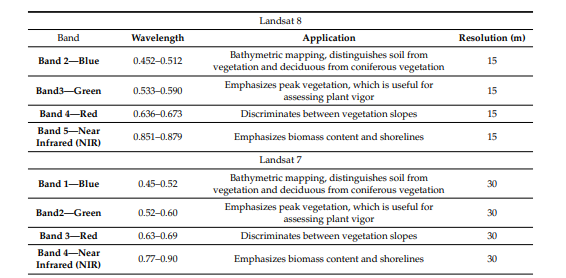
\includegraphics[width=0.7\linewidth]{./wavelength-9.png}
	\caption{Landsat Satellite Sensor characteristics}
	\label{fig:wavelength}
\end{figure}

\section{Methodology}
As undergraduate students with limited knowledge and expertise, we were not able to come up with a novel idea. However, keeping in mind the techniques learned in the course of Applied Digital Image Processing, we implemented the methods that have been used for detecting deforestation in the papers cited above.

\subsection[4.1]{Data Collection}
We acquired the satellite images from Google Earth Pro that is available for free from Google. For the multiple band images, we used Landsat 8 images from the USGS Earth Explorer website. The images were downloaded in the GeoTIFF format and were used for further processing. The images taken and uploaded on our Github repository are from the rural and urban areas of Sindh. 

\subsection[4.2]{Feature Extraction}
When it comes to images obtained from Google Earth Pro, we applied Fuzzy C-Mean Clustering (refer to Section 3.1) and Otsu thresholding (refer to section 3.2) separately. 

For the multi-band images, we used the NDVI method (refer to section 3.4) and the Wavelength method (refer to section 3.5) separately.

\subsection[4.3]{Classification}
For comparing the results produced by the methods above, we used accuracy parameters and visual observation to determine the best method. The accuracy parameters used were precision, recall, and fScore. The visual observation was done by comparing the results produced by the methods with the ground truth images.

We also used parameters like timing the execution or running time of our programs to see which program runs faster. 

\section{Results}

\section{Conclusion}

\bibliographystyle{IEEEtran}
\bibliography{references.bib}
\end{document}